\section{源码测试}

\subsection{随机测试}
\begin{figure}[H]
    \vspace{-0.5em}
	\centering
	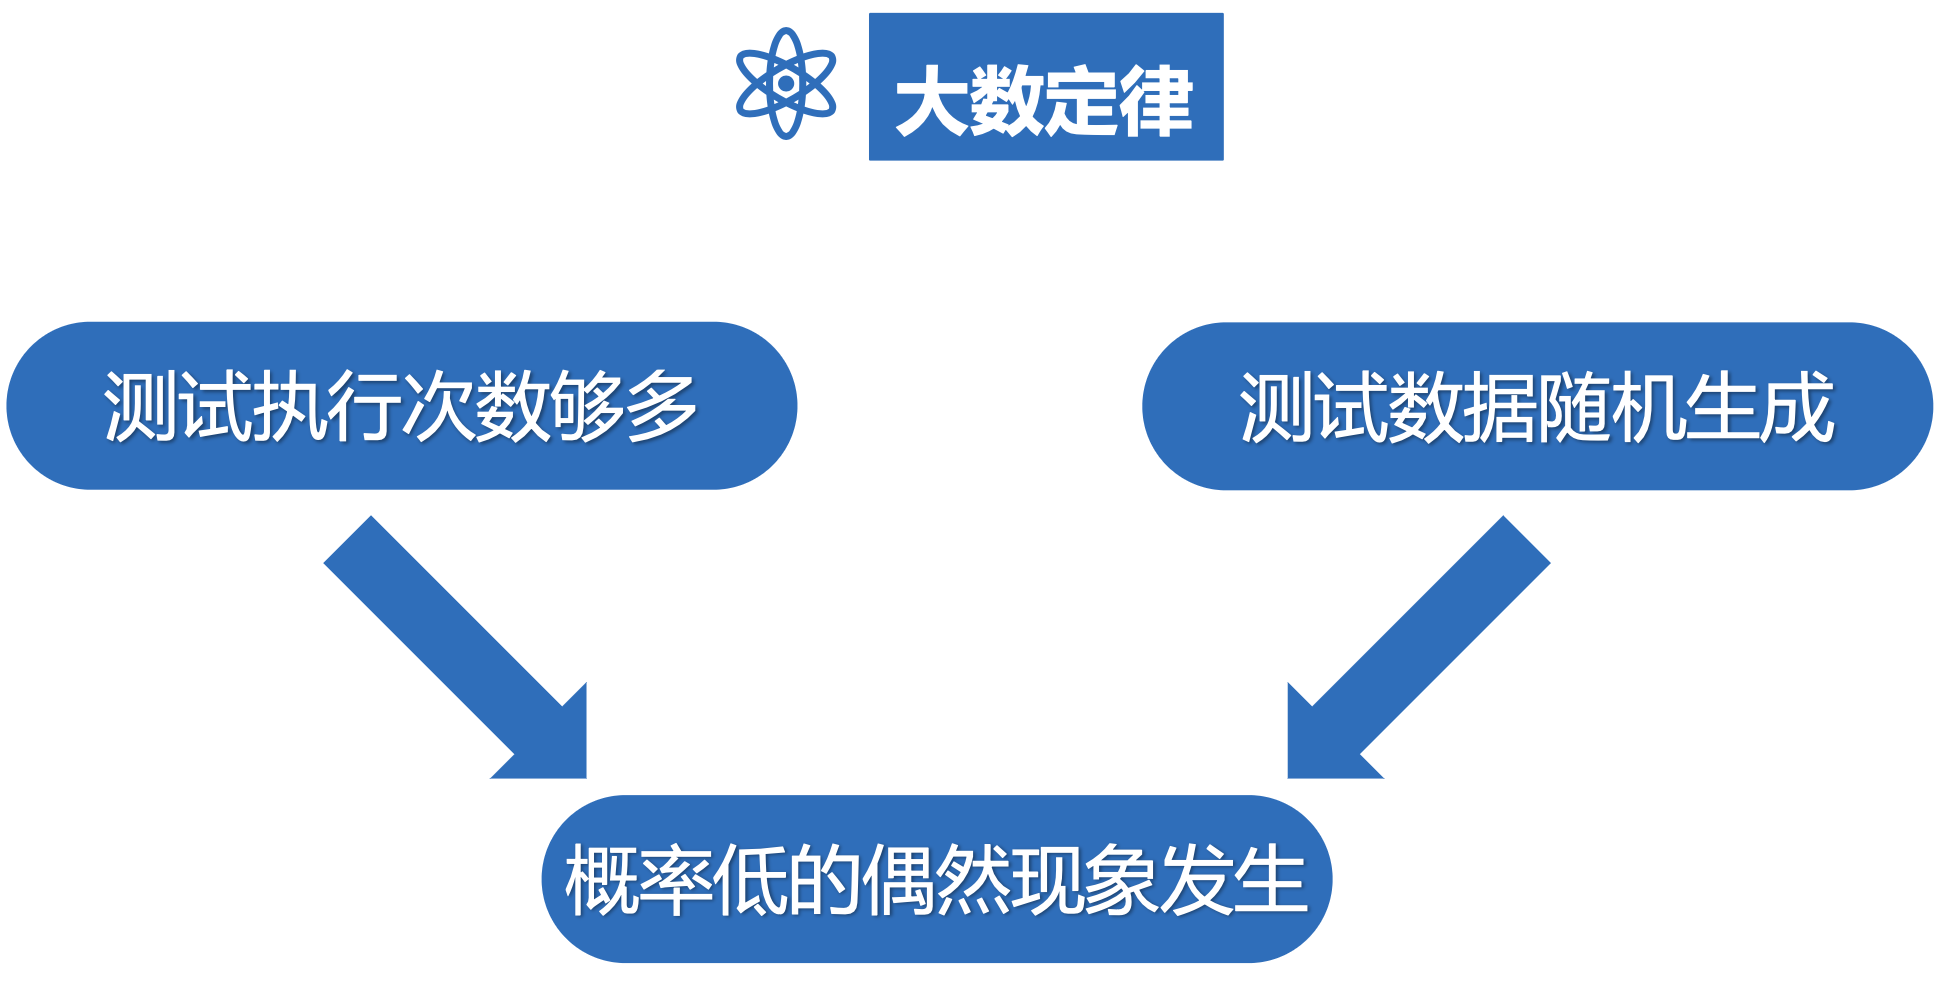
\includegraphics[width=0.5\textwidth]{images/随机测试.png}
    \vspace{-1em}
\end{figure}

\subsection{变异测试}
变异测试旨在找出有效的测试用例,发现程序中真正的错误。
\begin{figure}[H]
    \vspace{-0.5em}
	\centering
	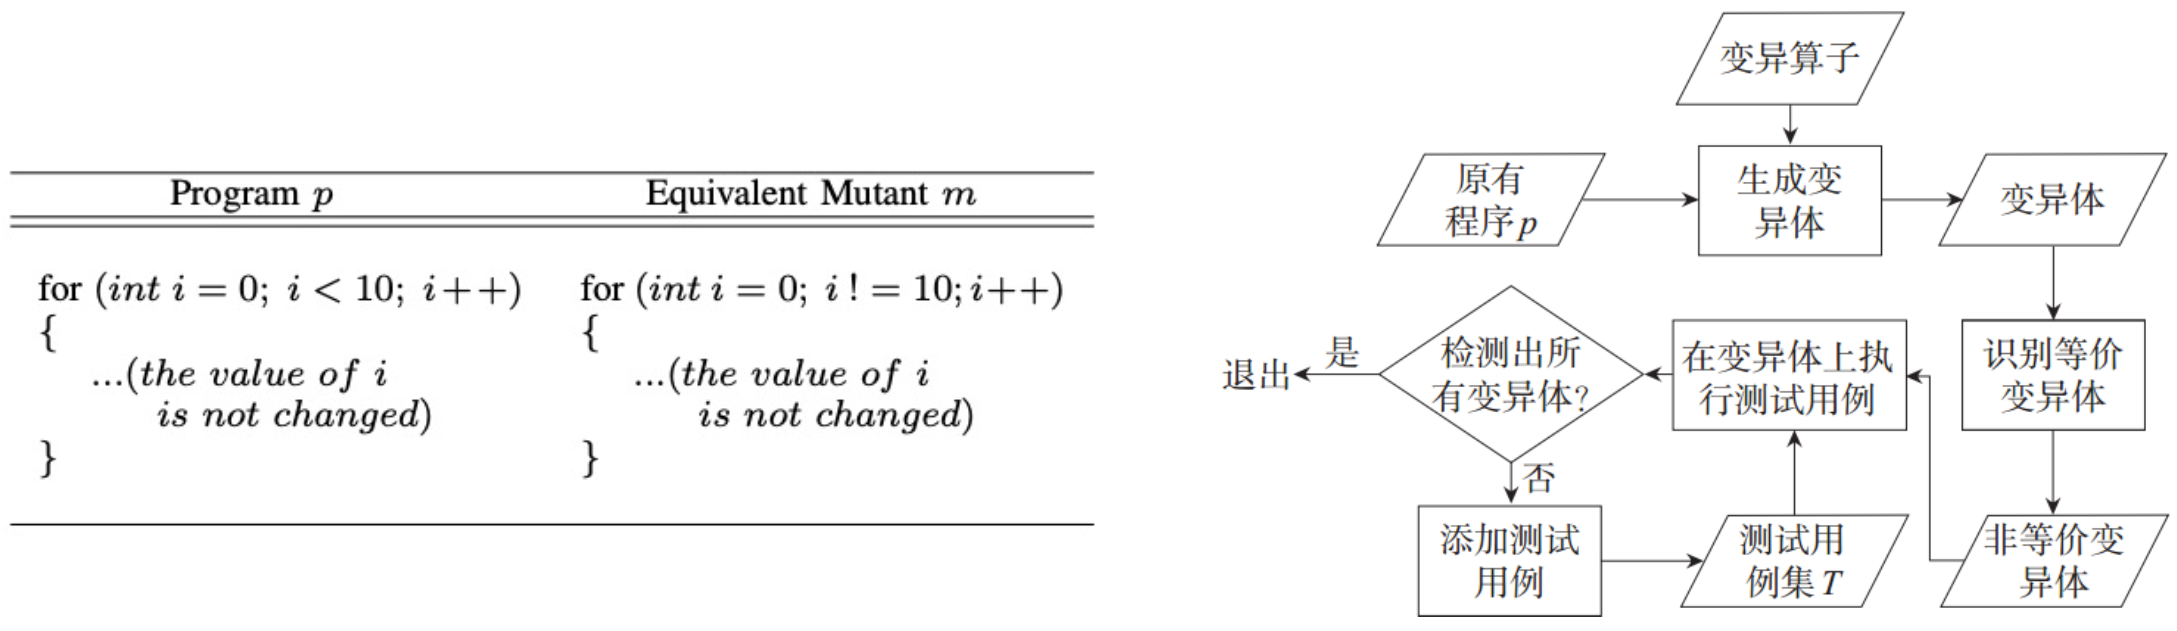
\includegraphics[width=0.95\textwidth]{images/变异测试.png}
    \vspace{-1em}
\end{figure}

\subsection{差分测试}
基本思想:通过将同一测试用例运行到一系列相似功能的应用中观察执行差异来检测bug。
\begin{figure}[H]
    \vspace{-0.5em}
	\centering
	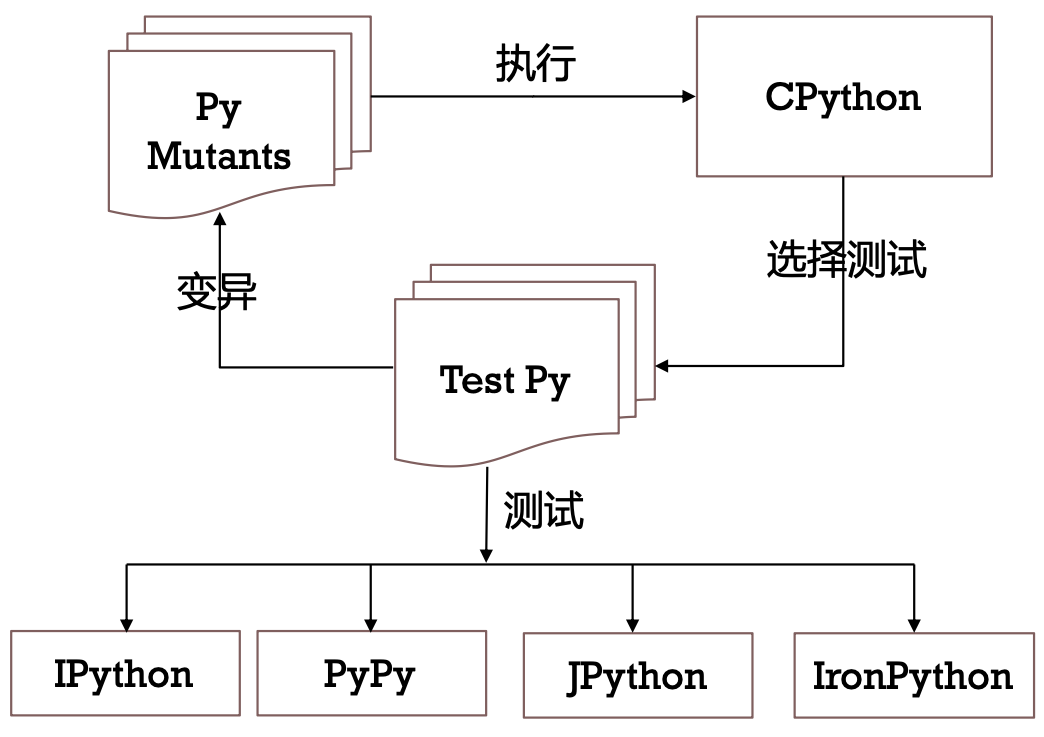
\includegraphics[width=0.4\textwidth]{images/差分测试.png}
    \vspace{-1em}
\end{figure}

\subsection{蜕变测试}
蜕变关系(Metamorphic Relation, MR)是指多次执行目标程序时,输入与输出之间期望遵循的关系。
\begin{figure}[H]
    \vspace{-0.5em}
	\centering
	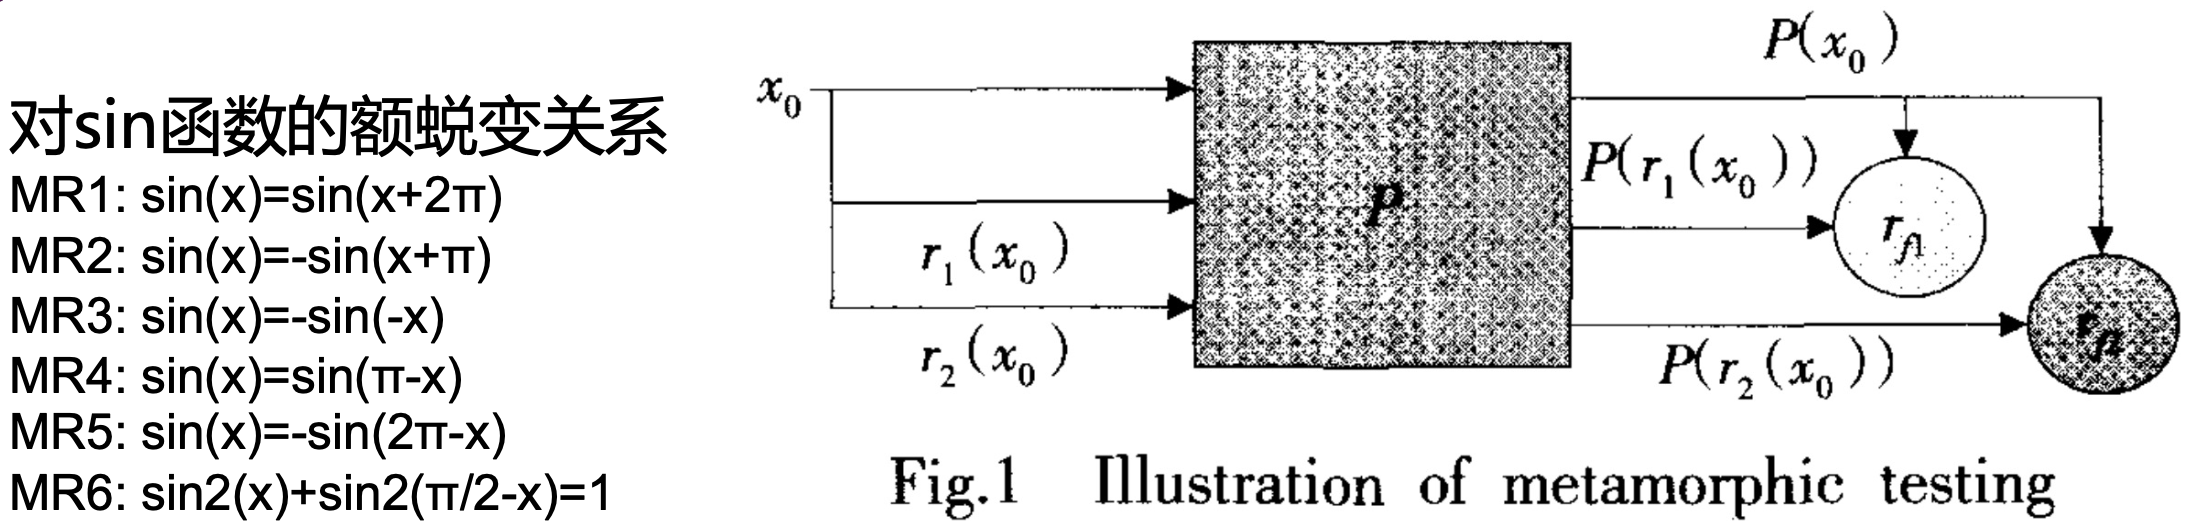
\includegraphics[width=0.75\textwidth]{images/蜕变测试.png}
    \vspace{-1em}
\end{figure}

\subsection{测试用例优先级(TCP)}

测试用例优先级的定义:通过设定特定优先级准则(执行时间,代码覆盖等),对测试用例进行优先级排序以优化其执行次序,旨在最大化优先级目标,例如最大化测试用例集的早期缺陷检测速率。

优先级策略:
\begin{itemize}
    \item 基于贪心的TCP策略
    \item 基于相似性的TCP策略
    \item 基于搜索的TCP策略
    \item 基于机器学习的TCP策略
\end{itemize}

\subsubsection{基于贪心的TCP策略}

\begin{itemize}
    \item 全局贪心策略
    \begin{itemize}
        \item 每轮优先挑选覆盖最多代码单元的测试用例
        \item 多个用例相同随机选择
    \end{itemize}
    \item 增量贪心策略
    \begin{itemize}
        \item 每轮优先挑选覆盖最多,且\textbf{未被已选择用例覆盖代码}单元的测试用例
        \item 所有代码单元均已被覆盖则重置优先级排序过程
        \item 多个用例相同随机选择
    \end{itemize}
\end{itemize}

\begin{figure}[H]
    \vspace{-0.5em}
	\centering
	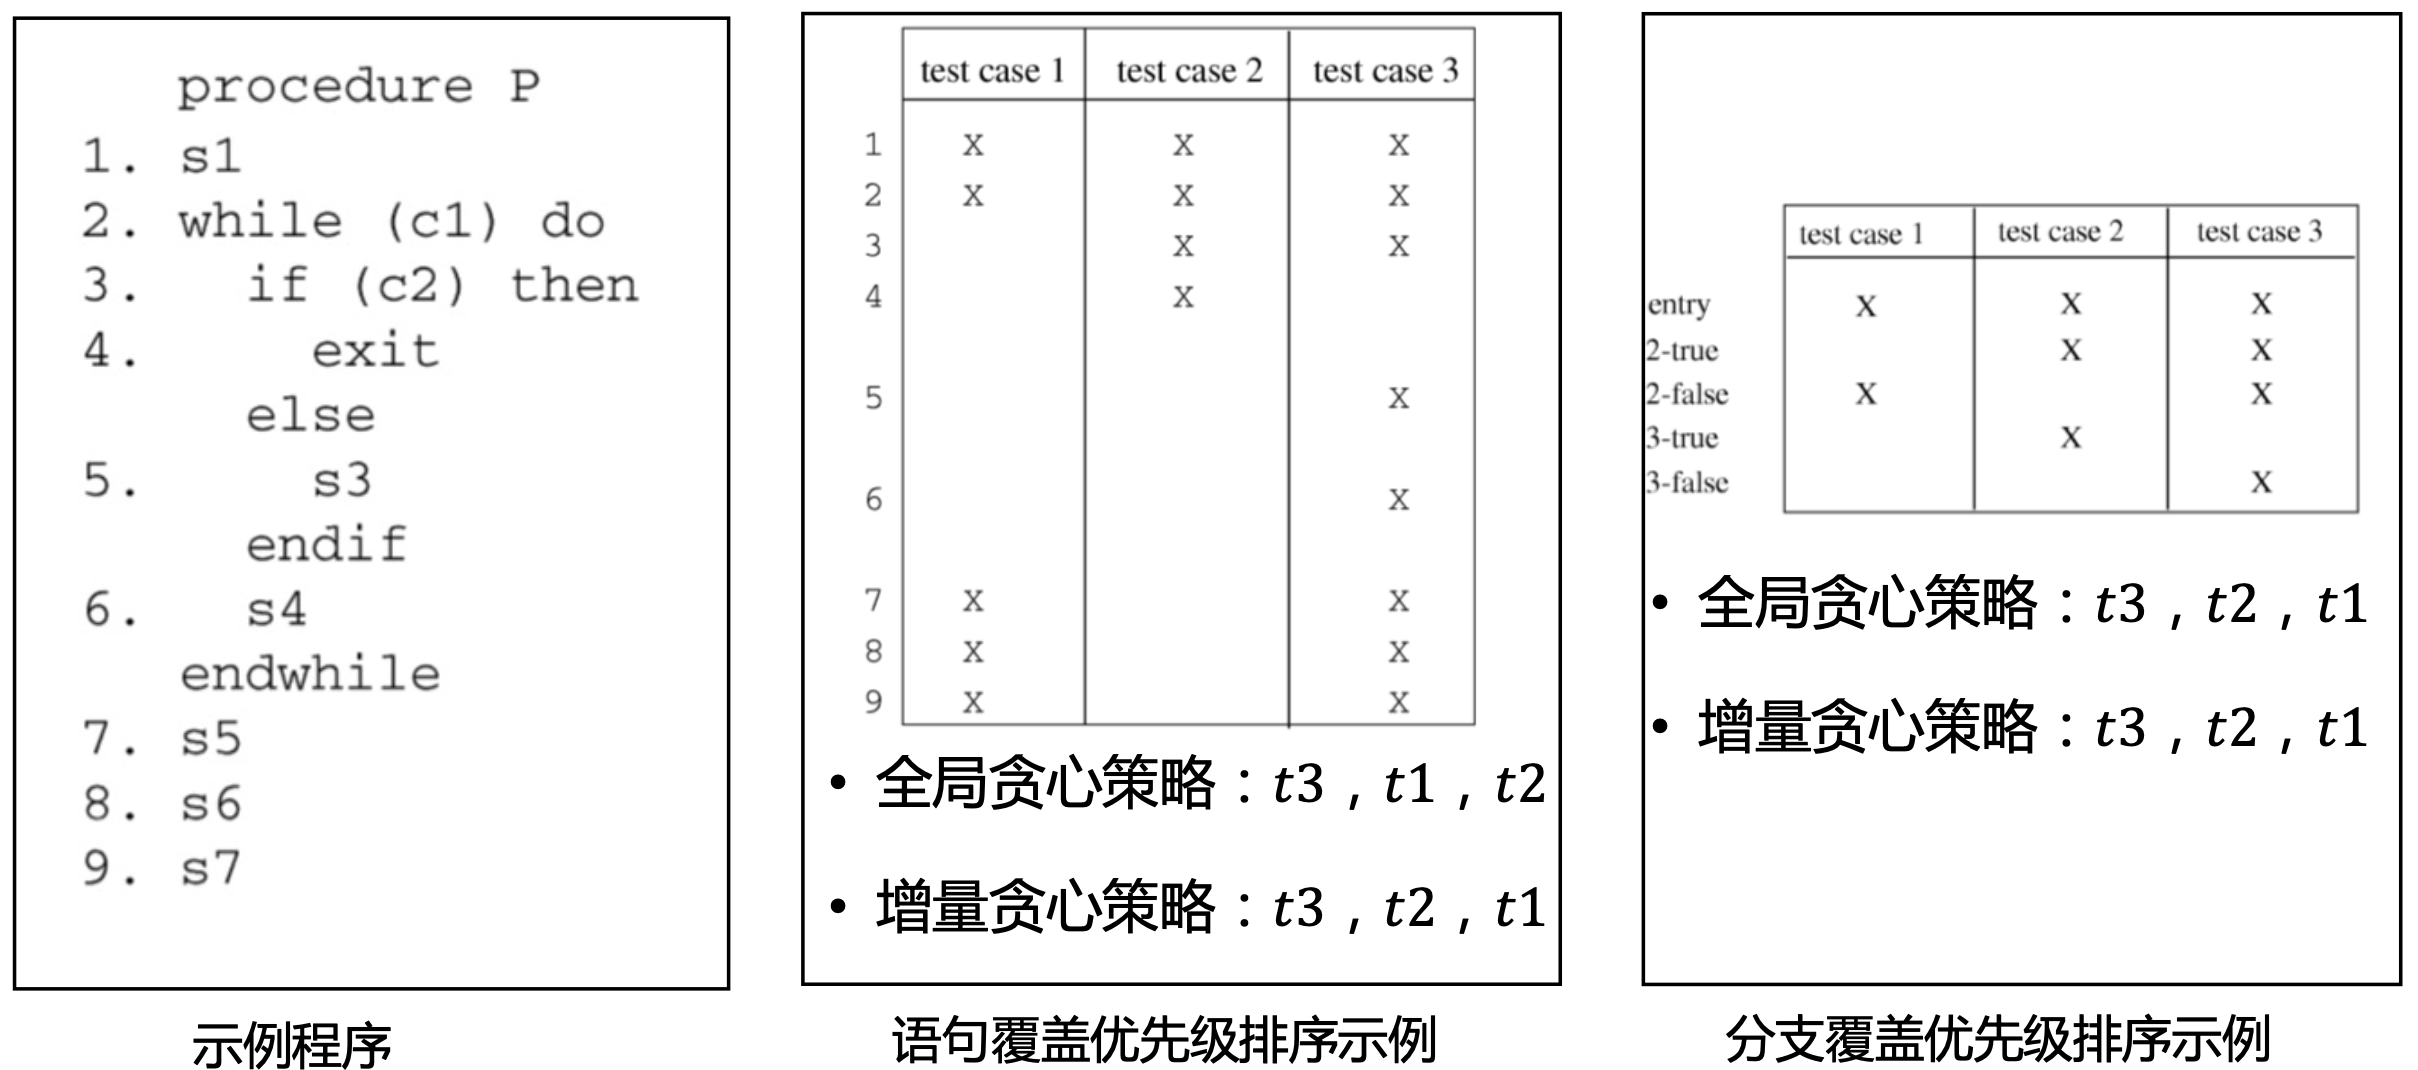
\includegraphics[width=0.8\textwidth]{images/基于贪心的TCP策略.png}
    \vspace{-1em}
\end{figure}

计算过程:
\begin{enumerate}[label=\arabic*.]
    \item 初始化覆盖矩阵和语句覆盖数组,所有代码单元均未被覆盖,$c$为全0数组
    \begin{figure}[H]
        \vspace{-0.5em}
        \centering
        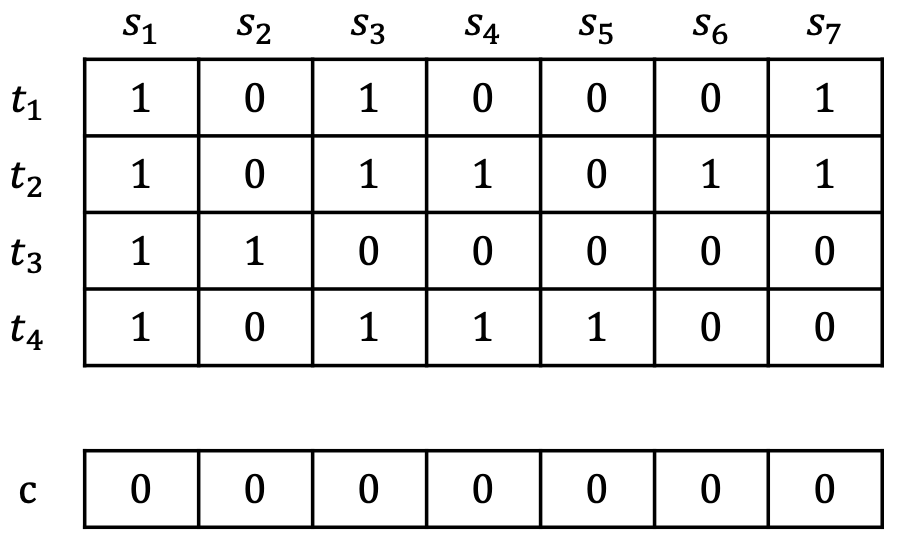
\includegraphics[width=0.3\textwidth]{images/基于贪心的TCP策略计算过程.png}
        \vspace{-1em}
    \end{figure}
    \item 根据覆盖矩阵和单元覆盖数组,计算待排序用例覆盖值,选择测试用例
    \item 选择测试用例,更新语句覆盖数组,以及待排序测试用例覆盖值
    \item 重复上述步骤,当所有语句均被覆盖时,重置语句覆盖数组,计算剩余测试用例覆盖值
\end{enumerate}

假设有$n$个测试用例以及$m$个代码单元,共需排序$n$轮,每轮选择一个测试用例,第$k$轮时,存在$n-k+1$个待排序用例,每个用例需与$m$个代码单元计算情况,那么时间复杂度为$O(n^2m)$。

\subsubsection{基于相似性的TCP策略}
自适应随机策略:每轮优先与已选择测试用例集差异性最大的测试用例。让测试用例均匀地分布在输入域中。

测试用例之间的距离计算:假设$U(t_1)$和$U(t_2)$为测试用例$t_1$和$t_2$所覆盖的代码单元集合,那么这两个用例之问的距离计算如下:
$$Jaccard(t_1, t_2) = 1-\frac{|U(t_1) \cap U(t_2)|}{|U(t_1) \cup U(t_2)|}$$

测试用例与测试用例集之间的距离计算:分别使用最小距离、平均距离和最大距离度量方式计算待选择用例$t_c$与已选择用例集$S$的距离:
$$
D(t_c, S) = \left\{ \begin{array}{c}
    \max\{\min\limits_{0\leq i \leq |S|} \{Jaccard(t_c,t_i)\}\} \\
    \max\{\mathop{\mathrm{avg}}\limits _{0\leq i \leq |S|} \{Jaccard(t_c,t_i)\}\} \\
    \max\{\max\limits_{0\leq i \leq |S|} \{Jaccard(t_c,t_i)\}\} \\
\end{array}\right.
$$

\begin{figure}[H]
    \vspace{-0.5em}
	\centering
	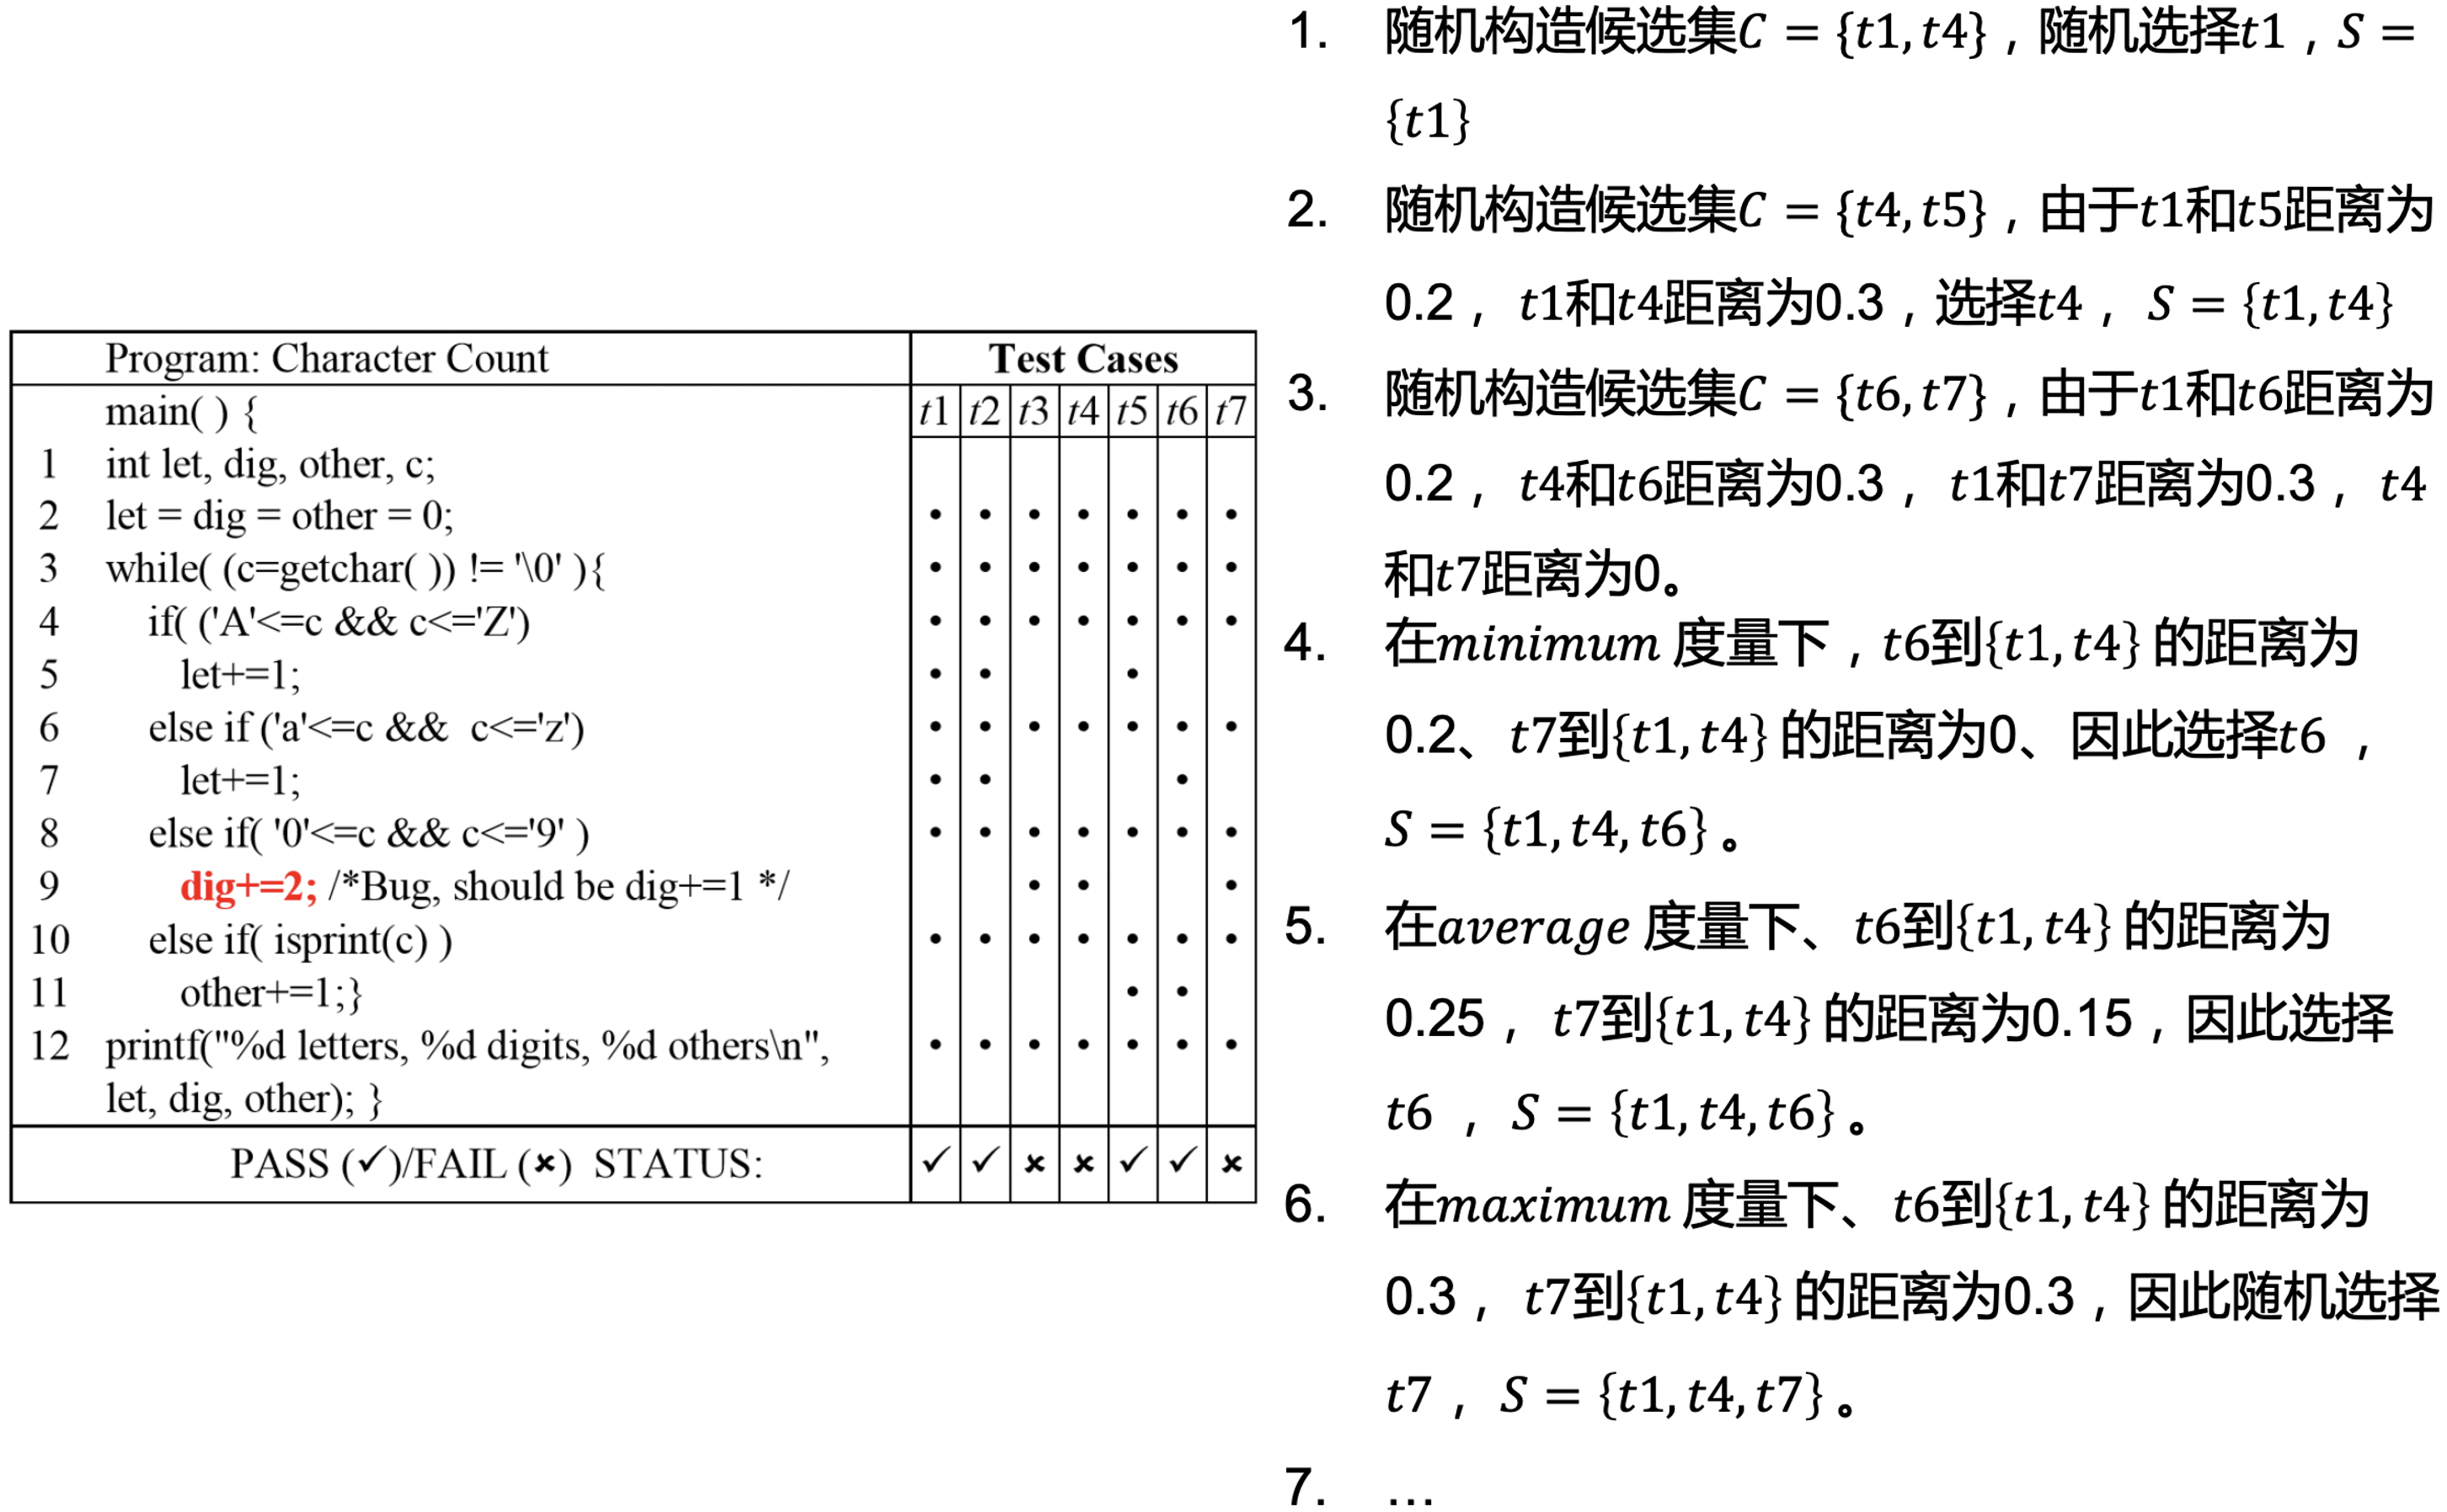
\includegraphics[width=0.75\textwidth]{images/基于相似性的TCP策略.png}
    \vspace{-1em}
\end{figure}

\subsubsection{基于搜索的TCP策略}
探索用例优先级排序组合的状态空间,以此找到检测错误更快的用例序列
\begin{itemize}
    \item 初始种群构造:测试用例位置构成解编码形式。
    \item 交叉操作:使用单点交叉方式,交换两个用例切割点前后部分。
    \item 变异操作:随机选取个体中的两个基因座进行交换。
    \item 适应度评估:使用用例序列的覆盖代码单元速率进行评估
\end{itemize}

\subsubsection{基于机器学习的TCP策略}
对测试用例特征进行学习,根据预测的缺陷检测概率进行优先级排序。
\begin{enumerate}[label=\arabic*.]
    \item 特征提取:设计并提取测试程序中源码特征。
    \item 缺陷模型:建立模型预测测试程序检测缺陷的概率。
    \item 开销模型:建立模型预测测试程序的运行时问。
    \item 测试优先级:基于单位时间内检测缺陷能力进行优先级排序。
\end{enumerate}

\subsubsection{APFD计算}
APFD的一般性描述:给定程序包含$m$个故障$F=\{f_1,f_2,\cdots, f_m\}$和$n$个测试用例$T=\{t_1,t_2,\cdots, t_n\}$,$T^ \prime$为$T$的一个优先级序列,$TF_i$为该测试用例序列$T^ \prime$中第一个检测到故障$f_i$的测试用例下标,则该优先级序列$T^ \prime$的APFD值计算公式为
$$APFD=1- \frac{TF_1 + TF_2 +\cdots + TF_m}{n\times m} + \frac{1}{2n}$$

\begin{figure}[H]
    \vspace{-0.5em}
	\centering
	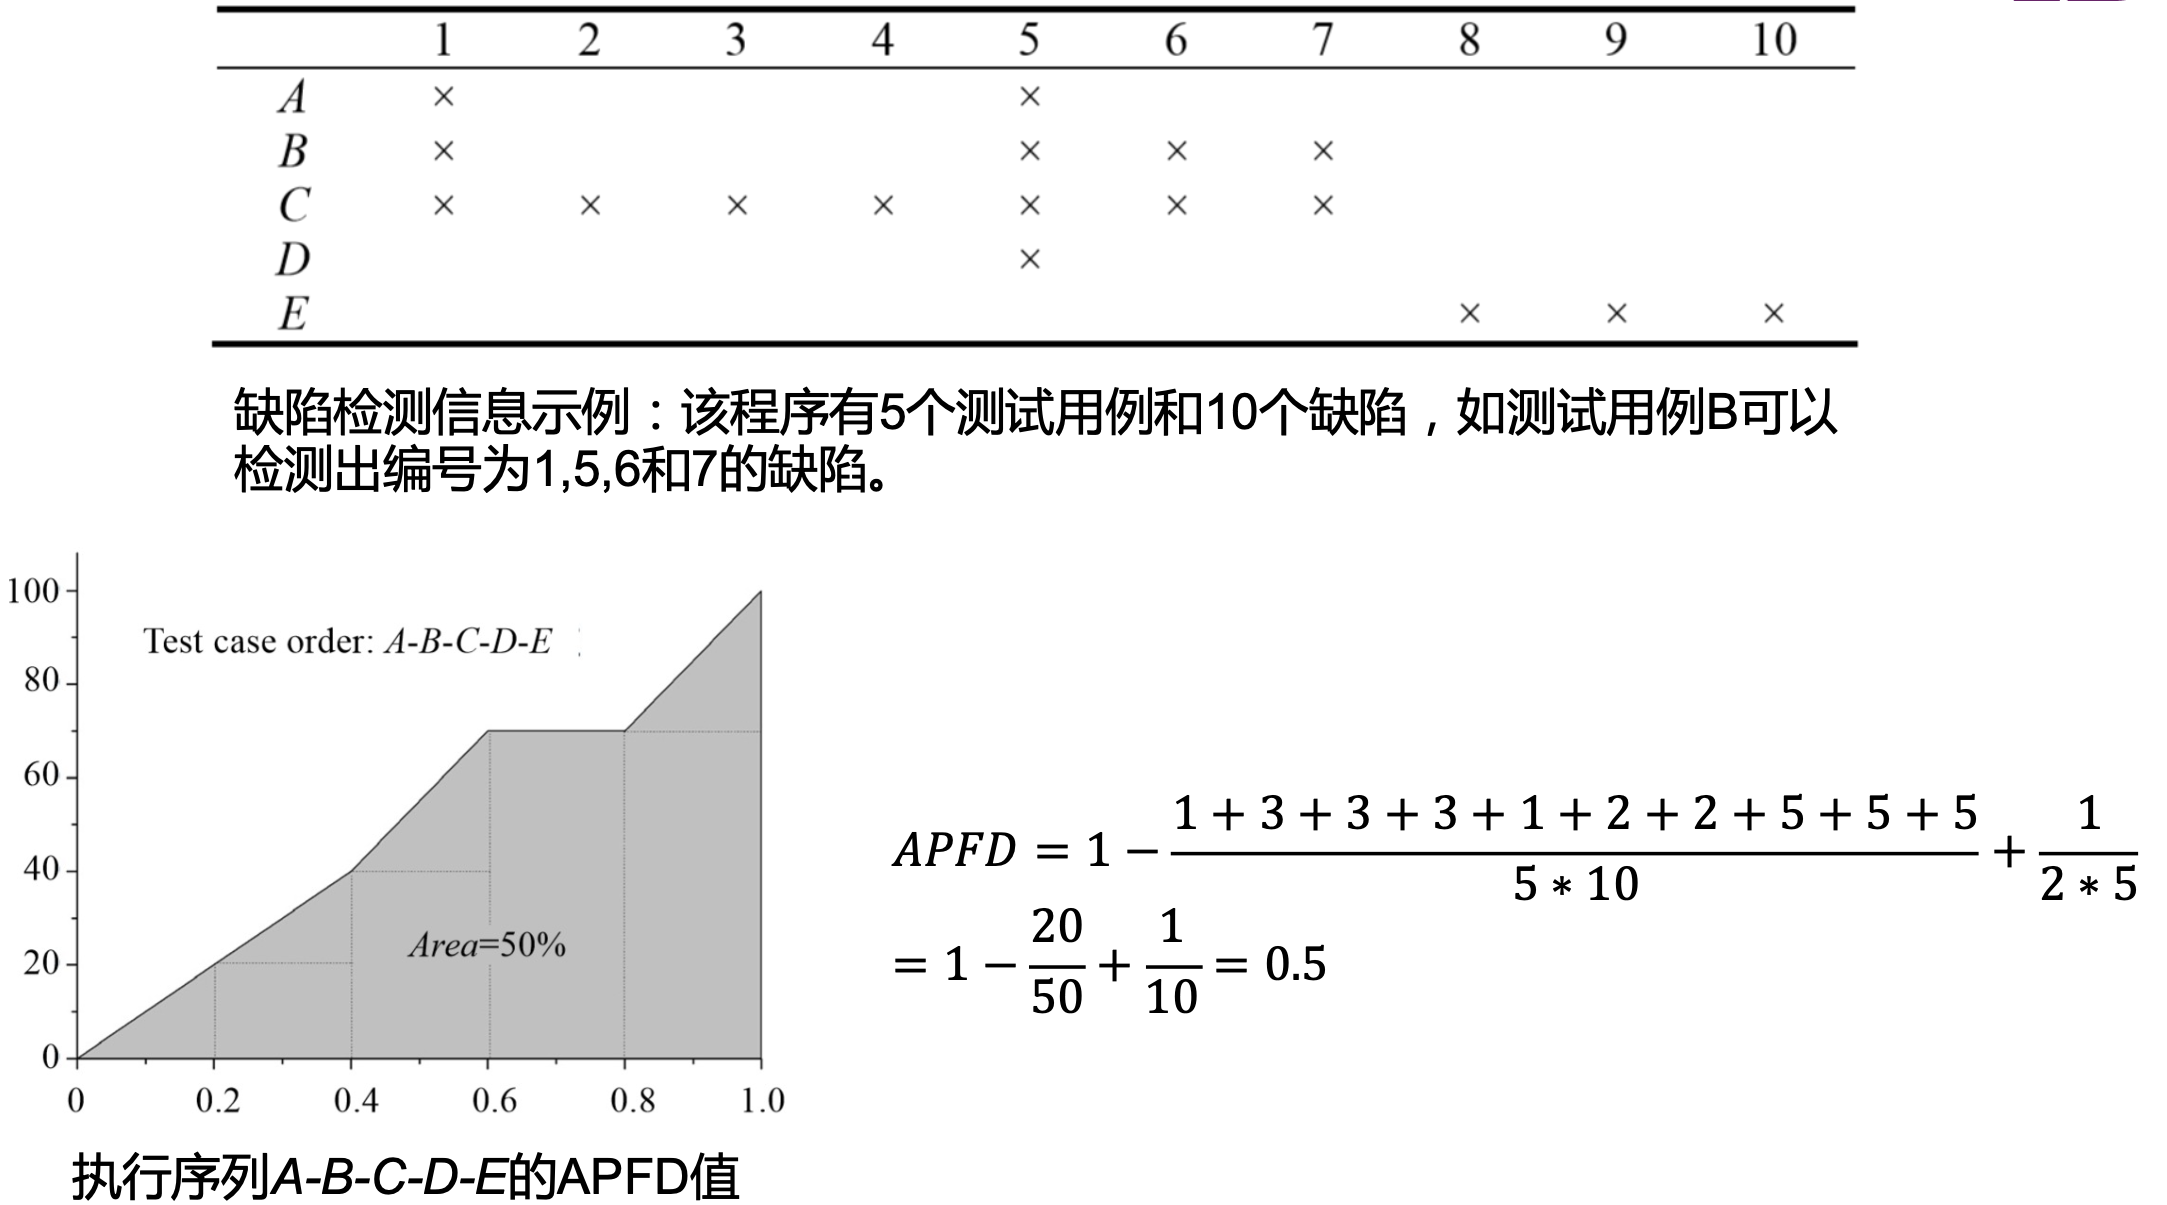
\includegraphics[width=0.8\textwidth]{images/APFD.png}
    \vspace{-1em}
\end{figure}

\subsection{测试用例选择(TCS)}
TCS定义:旨在从已有测试用例集中选择出所有可检测代码修改的测试用例。

适用场景:适用于因测试预算不足以致不能执行完所有测试用例的测试场景。

测试选择是回归测试选择的核心环节
\begin{itemize}
    \item 测试选择可以依照某种策略,从测试全集中筛选出一个子集。通过重新运行这个一个子集,验证版本迭代是否对软件既有的某些功能造成了影响。
    \item 给定修改前的生产代码$P$、修改后的生产代码$P^\prime$以及测试全集$T$,测试选择就是根据某种选择策略$S$,从$T$中筛选出测试子集$T^\prime$,使$T^\prime$能够评估代码变更是否影响了程序的既有功能。
\end{itemize}

根据不同的选取策略,测试用例选择可大致分为以下四类
\begin{itemize}
    \item 最小化测试用例选择技术
    \begin{itemize}
        \item 目标:从原测试套件$T$中选出最少的测试用例组成最小最小测试集$T_{min}$ ,使得产生的$T_{min}$能多覆盖被测程序$P$中所有本次修改的、或者受本次修改影响的部分。
        \item 要求:一个最小化测试用例选择技术要求修改后的被测试程序$P$中,每一条新增的或者被修改的语句都能够被至少一个来自原测试套件$T$的测试用例执行。
    \end{itemize}
    \item 安全测试用例选择技术
    \begin{itemize}
        \item 目标:针对某种特定的测试需求,选取出源测试套件$T$中所有能够暴露修改后被测程序$P^\prime$中的一个或多个缺陷的所有测试用例,构成安全回归测试集$T_S$。
        \item 一个安全测试用例选择技术要求在目标程序$P$运行回归测试时,$T_S$中的每个测试都能够满足以下条件之一:
        \begin{itemize}
            \item 执行至少一条在$P^\prime$中被删除的语句
            \item 执行至少一条在$P^\prime$中新增的语句
        \end{itemize}
    \end{itemize}
    \item 基于数据流和覆盖的测试用例选择技术
    \begin{itemize}
        \item 目标:当代码变更发生后,原待测程序$P$更新为$P^\prime$。相比于$P$,$P^\prime$中部分语句的数据交互发生了变化。这些发生变化的语句构成了语句集合$S_I$。基于数据流和覆盖的测试用例选择技术的目标是选取出所有能够执行到$S_I$中某条语句的测试用例,组成测试集$T_D$。
        \item 要求:一个安全测试用例选择技术要求在目标程序$P$运行回归测试时,$T_D$中的每个测试都能够满足以下条件之一:
        \begin{itemize}
            \item 执行至少一个在$P^\prime$中被删除的Define-Use对
            \item 执行至少一个在$P^\prime$中新增的Define-Use对
        \end{itemize}
    \end{itemize}
    \item 特制/随机测试用例选择技术
    \begin{itemize}
        \item 定义:当时间不允许使用ReTestAl策略进行回归测试、且没有任何可用的测试用例选择工具时,开发人员通常会依赖“直觉"或者测试与生产代码功能之间的弱关联进行测试用例选择。
        \item 举例:
        \begin{itemize}
            \item 随机测试用例选择:规定测试用例的选取数量为$m$ ,测试人员随机地从原始测试套件$T$选出$m$个测试用例,组成随机回归测试集$T_R$
            \item 面向剖面测试用例选择:与面向剖面程序编程有关,从原始测试套件$T$中选出与某个剖面$a$有关的化测试用例,组成回归测试集$T_a$
        \end{itemize}
    \end{itemize}
\end{itemize}

\subsection{基于程序分析的测试选择}
一种依赖程序分析的测试选择技术。该技术一般通过程序分析技术计算测试代码(方法、用例或套件)与生产代码之间存在的依赖关系,井在代码发生变更时,利用这些依赖关系将所有受到变更影响的测试代码自动选取出来,组成测试子集。

\begin{itemize}
    \item 静态测试选择:以静态程序分析为基础实现的测试选择技术。静态(程序)分析是指在没有实际执行程序的情况下对计算机软件程序进行自动化分析的技术。
    \item 动态测试选择:以动态程序分析为基础实现的测试选择技术。动态(程序)分析通过在真实或虚拟处理器上执行程序来完成对程序行为的分析。为了使动态程序分析有效,此须使用足够的测试输人来执行目标程序,以尽可能覆盖程序所有的输出。
\end{itemize}

对比动态测试用例选择和静态测试用例选择
\begin{itemize}
    \item 总体:动态测试用例选择>静态测试用例选择。
    \item 以面向Java语言的测试用例选择技术为例,动态测试用例选择技术一般要优于静态测试用例选择技术,原因在于:动态分析能够更容易地获得更加丰富的(运行时信息)程序依赖信息,测试用例选择更加精准、安全;而相比之下静态分析的开销更大,同时存在过拟合现象。
    \item 静态测试用例选择技术在运行测试阶段的表现一般要优于动态测试用例选择技术,其原因在于静态分析不需要对代码进行插桩 ,在执行代码前就能够获得测试用例选择所需的测试依赖。
\end{itemize}

类防火墙算法:所有能够通过继承边或使用边直接或间接到达某些发生变更类型的类型的集合
\begin{itemize}
    \item 给定一组变更的类,类防火墙将利用类之间的关系计算其他可能受变更影响的一组类,即围绕变更的类构建“防火墙”
\end{itemize}
\begin{figure}[H]
    \vspace{-0.5em}
	\centering
	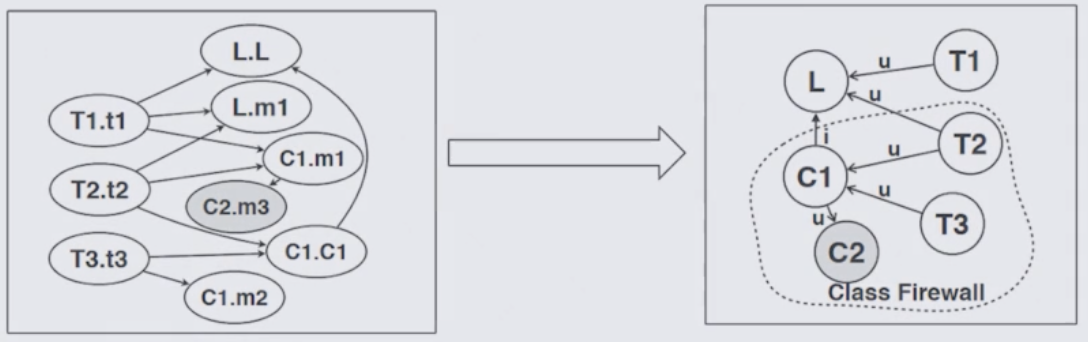
\includegraphics[width=0.6\textwidth]{images/类防火墙.png}
    \vspace{-1em}
\end{figure}

回归测试优先选择:
\begin{enumerate}[label=\arabic*.]
    \item 新修改的功能,这个显然是重点;
    \item 新修改的功能的关联功能,就是有耦合的部分,这个一般最好咨询一下开发人员;
    \item 程序最有卖点或者说亮点的部分,这个地方一旦有问题,会使程序质量大打折扣;
    \item 程序中最致命的部分,譬如说安全隐患,数据泄露,加密注册;
    \item 程序中比较脆弱的部分,这个要咨询开发人员,一般就是他们心中最没底的地方;
    \item 程序的主干功能;
    \item 如果以上做完,还有时间的话,最好把用例中级别比较高的用例再执行一遍。
\end{enumerate}

\subsection{TCP和TCS的对比}
测试用例选择:通过分析代码修改,从已有测试用例中选择出所有可检测代码修改的测试用例,并确保未被选择的测试用例在修改前后程序上的执行行为保持一致。

测试用例优先级:当测试预算不足以执行完所有测试用例时,基于特定的优先级准则,对测试用例进行优先级排序,以优化其执行次序,旨在最大化优先级目标。

